The project uses C++ as the language and Qt-framework to make things easier and manageable. There are other technologies that have been used and are discussed further. Currently, no database have been used for this project. But we may incorporate database in our project to make it more robust and extensible.

After studying about some existing systems or libraries to read/write DXF files we came to a conclusion and choose a library 'dxflib'. It is an open-source library under development by QCAD. It supports reading and writing DXF files. The basic flow of the dxflib library is shown in the figure.


\begin{figure}
\centering 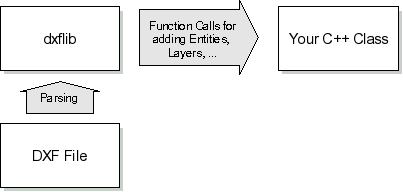
\includegraphics[scale=.9]{images/dxflib.png}
\caption{dxflib workflow}
\end{figure}


\section{Coding Outline}
The file structure of the project goes like this. There are mainly four files: a project.pro file, entity.cpp, entity.h and main.cpp.

\subsection*{pro file}
This is a Project file created for a Qt project. Project files contain all the information required by qmake to build your application, library, or plugin. The resources used by your project are generally specified using a series of declarations, but support for simple programming constructs allow you to describe different build processes for different platforms and environments.

\subsection*{entity.cpp}
This is the file where entities are defined. As of now, there are two entities: createWall and createFlange. There will be more entities definition in the future like beam, column, stairs etc.

\subsection*{entity.h}
It contains the function declaration for the entities like createWall etc. that have been used in the entity.cpp file later on.


\subsection*{main.cpp}
This is the main file. First of all, we need an input file say "in.txt" which will contain the something like:
wall(l=100,h=130,cx=10,cy=10). and it is then parsed by the main.cpp program using regular expressions to separate out the relevant information and stored in "out.txt" temporarily. Which is then parsed to create the entities using the library. If we talk about the input file. It contains a keyword "wall" which is pretty intuitive to guess that we are going to create a wall. Then there are four arguments where 'l' is for length of the wall, 'h' is for height of the wall and 'cx', 'cy' are the x and y coordinates of the starting point of the wall respectively.

Initially, the order in which the arguments are passed mattered. But now each of the following enitity will create the same drawing.
\begin{lstlisting}
wall(l=100,h=30,bx=10,by=10)

wall(h=50,l=120,bx=10,by=40)

wall(bx=20,h=100,by=100,l=60)
\end{lstlisting}


There is another library 'libdxfrw' which we found recently that is under more rapid development than dxflib. It is also an open-source library created by LibreCAD (An open-source community-based CAD software). It have support for newer versions of DXF and it have also support to read the DWG files. We may incorporate this library into our project.